\bookchapter{פרק 49: הקמת סביבת הפיתוח — Android Studio והפרויקט הראשון}

\chapterintro{לפני שעושים מלאכה טובה — משחיזים את הכלים. בפרק זה נקים את ה“מטבח”: נתקין את Android Studio, נריץ בהצלחה את האמולטור, ניצור את פרויקט האנדרואיד הראשון בחיים שלכם, ונפרק את מבנה הפרויקט לגורמים כדי להבין אותו היטב. אחרי שהסביבה מוקמה, תראו בפעם הראשונה את הקוד שכתבתם הופך לכפתור שאפשר ללחוץ עליו — רגע שרבים זוכרים כל החיים.}

\booksection{א. התקנת Android Studio}

Android Studio הוא סביבת הפיתוח המשולבת (IDE) הרשמית של Google — חינמית, עם חבילת פונקציונליות מלאה: כתיבת קוד, תצוגה מקדימה של הממשק, ניפוי שגיאות ואריזה — הכול בפנים. התקנה בארבעה צעדים:

\begin{enumerate}
  \item פתחו את האתר הרשמי developer.android.com/studio והורידו את הגרסה היציבה העדכנית (באוגוסט 2026 — הגרסה שאחרי Narwhal; זמינה ל-Windows/Mac/Linux);
  \item הריצו את קובץ ההתקנה ולחצו "הבא" שוב ושוב — אשף ההתקנה יכלול אוטומטית את Android SDK ואת רכיבי האמולטור;
  \item בהפעלה הראשונה הורידו את רכיבי ה-SDK לפי ההנחיות (ברירת המחדל מספיקה; זה עשוי לקחת כמה דקות וכמה GB של מקום);
  \item בסיום תגיעו למסך הפתיחה — מזל טוב, ה"מטבח" מוקם.
\end{enumerate}

\begin{tcbwarn}{שימו לב: היו מודעים לדרישות החומרה}
Android Studio הוא “בולען זיכרון”: מומלץ 16GB זיכרון ומעלה (8GB זה אפשרי, אבל האמולטור ירגיש מגושם), 20GB ומעלה של מקום בכונן, ומעבד שתומך בווירטואליזציה (הפעילו VT-x/AMD-V ב-BIOS). אם המחשב באמת ישן, אפשר להחליף את האמולטור ב“ניפוי שגיאות על מכשיר אמיתי” (נדבר על כך בסעיף 4 של הפרק) — והחוויה אף חלקה יותר.

\end{tcbwarn}

\booksection{ב. יצירת הפרויקט הראשון שלכם}

במסך הפתיחה לחצו New Project, בחרו בתבנית Empty Activity (התבנית הנקייה ביותר למתחילים) ומלאו שלושה פרטים:

\begin{center}
\begin{tabularx}{\linewidth}{|X|X|X|}
\hline
\textbf{שדה הגדרה} & \textbf{מה ממלאים} & \textbf{הסבר} \tabularnewline
\hline
Name & My First App & שם האפליקציה — מוצג במסך הבית של הטלפון \tabularnewline
Package name & com.example.myfirstapp & מזהה ייחודי בעולם; הנוהג הוא "שם דומיין הפוך" — לעת עתה השאירו את ברירת המחדל \tabularnewline
Minimum SDK & API 26(Android 8.0) & גרסת התמיכה המינימלית — מכסה 95\%+ מהמכשירים \tabularnewline
\hline
\end{tabularx}
\end{center}

\begin{center}\small\color{gray}שלושת הפרטים שממלאים ביצירת פרויקט\end{center}

אחרי לחיצה על Finish, Android Studio יוריד אוטומטית את התלויות ויבנה את הפרויקט באמצעות Gradle (בפעם הראשונה זה לוקח כמה דקות; אחר כך מהר הרבה יותר). עם סיום הבנייה, יש לכם אפליקציה רצה — גם אם לעת עתה היא רק מציגה שורת “Hello Android!”.

\begin{tcbinfo}{טיפ: סודות שם החבילה}
שם החבילה (package name) הוא בעצם “מספר תעודת הזהות” של האפליקציה — ייחודי ברחבי העולם, ואי אפשר לשנות אותו אחרי העלייה לחנות. לתרגול אישי com.example.xxx מספיק; למוצר רשמי יש להחליף לשם הדומיין ההפוך שלכם (למשל com.<השם שלכם>.<שם האפליקציה>). אל תעלו לחנות עם com.example — החנות תדחה זאת.

\end{tcbinfo}

\booksection{ג. להריץ: אמולטור ומכשיר אמיתי}

הקוד כתוב — עכשיו צריך “טלפון” שיריץ אותו. יש לכם שתי אפשרויות:

\booksubsection{האמולטור (Emulator)}

האמולטור מדמה טלפון אנדרואיד בתוך המחשב. ב-Android Studio פתחו Device Manager Create Device, בחרו מכשיר (מומלצת סדרת Pixel) בחרו תמונת מערכת (אחת עם Google APIs) הורידו הפעילו. אחר כך לחצו על המשולש הירוק Run בסרגל הכלים, ותוך כמה שניות האפליקציה שלכם תופיע על מסך ה“טלפון”.

\booksubsection{ניפוי על מכשיר אמיתי (מומלץ יותר)}

מכשיר אמיתי תמיד יהיה סביבת הבדיקה האמיתית ביותר — תחושת ההחלקה, רשת אמיתית, חיישנים אמיתיים; האמולטור לא משתווה. ניפוי על מכשיר אנדרואיד אמיתי הוא פשוט:

\begin{enumerate}
  \item בטלפון פתחו [הגדרות] [אודות הטלפון], הקישו 7 פעמים רצופות על "מספר הגרסה" (Build number) כדי להפעיל את "אפשרויות מפתח";
  \item בתוך [אפשרויות מפתח] הפעילו ניפוי USB (USB debugging);
  \item חברו את הטלפון למחשב בכבל נתונים, ובחלונית שתופיע בטלפון בחרו "אפשר ניפוי USB";
  \item חזרו ל-Android Studio — הטלפון שלכם יופיע ברשימת המכשירים בסרגל הכלים; לחצו Run.
\end{enumerate}

\textbf{אזהרת מלכודת: אל תשאירו ניפוי USB מופעל כל הזמן}\par

ניפוי USB הוא בעצם להשאיר “דלת אחורית” פתוחה למחשב. בטעינה במקומות ציבוריים ובחיבור למחשבים שאינכם סומכים עליהם — הקפידו לכבות ניפוי USB, כדי שאף אחד לא יוכל לקרוא את הנתונים שלכם דרכו. סגרו אותו מיד אחרי כל סבב פיתוח — פתחו הרגל.

\booksection{ד. פירוק מבנה הפרויקט: מה תפקידו של כל קובץ}

בפתיחה הראשונה של הפרויקט, עץ הקבצים משמאל עלול להסחרר. אל דאגה — בפיתוח השוטף, 90\% מהזמן תעבדו רק עם הפריטים הבאים:

\begin{center}
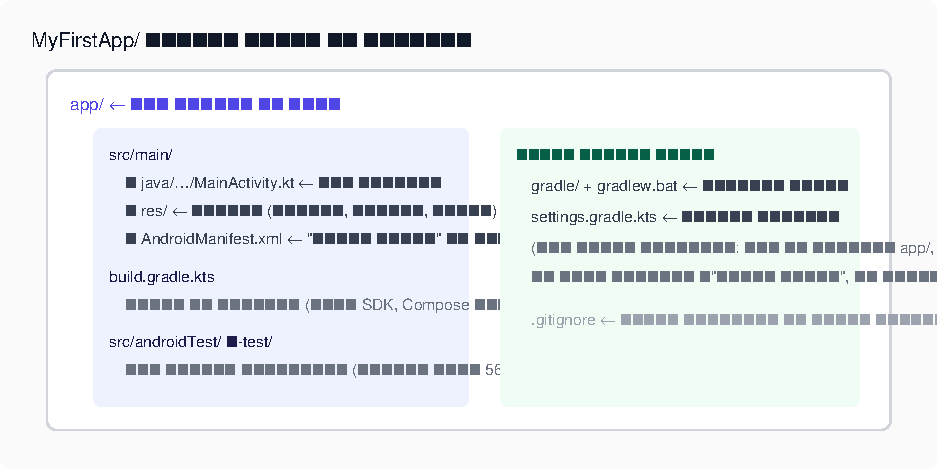
\includegraphics[width=0.92\linewidth]{figures/fig-di-si-shi-jiu-zhang-1}
\\[2pt]\small איור 2: מבנה הפרויקט שכל מתחיל חייב להכיר (כלל הזהב: נגיעה רק בתיקיית app/)
\end{center}

\begin{itemize}
  \item MainActivity.kt: "הדלת הראשית" של האפליקציה. כשהמשתמש לוחץ על הסמל, זה הראשון שמתעורר. בתבנית הנוכחית הוא אחראי להציג את "Hello Android!".
  \item AndroidManifest.xml: "רישום האוכלוסין" של האפליקציה — מצהיר מה שם האפליקציה, איזה סמל יש לה, אילו מסכים קיימים בה ואילו הרשאות היא דורשת (מצלמה, מיקום ועוד).
  \item תיקיית res/: מחסן המשאבים — שם נשמרים תמונות, סמלים, מחרוזות וצבעים. לשים טקסטים בקובצי משאבים ולא לקבע אותם בקוד זה נוהג טוב בפיתוח אנדרואיד (קל להחליף שפה או ערכת נושא).
  \item build.gradle.kts: מתכון הבנייה — מצהיר על גרסת התמיכה המינימלית ועל הספריות שהפרויקט תלוי בהן (למשל Compose).
\end{itemize}

\booksection{ה. טעימה ראשונה: להחליף את ה-“Hello” בשם שלכם}

פתחו את MainActivity.kt ותראו את הקוד שהתבנית של Compose ייצרה. מצאו את השורה Text(“Hello Android!”) החליפו את הטקסט שבמרכאות בשם שלכם, למשל Text(“שלום, ישראל! זו האפליקציה הראשונה שלי”), והריצו מחדש עם Ctrl+R (ב-Mac: Cmd+R). תוך כמה שניות שמכם יופיע על האמולטור.

\begin{lstlisting}[language=Kotlin]
setContent {
    MyFirstAppTheme {
        Surface(modifier = Modifier.fillMaxSize()) {
            // v שנו כאן לטקסט שלכם
            Text("שלום דני! זו האפליקציה הראשונה שלי")
        }
    }
}
\end{lstlisting}

מזל טוב — השלמתם מעגל מלא של “שינוי קוד הידור התקנה הרצה”. המעגל הזה הוא השגרה היומיומית של הפיתוח מעכשיו. בזמן שהברזל חם — נסו לשנות עוד משהו: הגדילו את הגופן, החליפו צבע — בפרק הבא נלמד מאיפה מגיעים ה“קסמים” האלה.

\booksection{ו. עזרה ראשונה לשגיאות נפוצות: “חדר המיון” של השבועיים הראשונים}

בשלב הקמת הסביבה והבנייה הראשונה, כנראה שתיתקלו בשלוש השגיאות הבאות. אל דאגה — לכולן יש תרופה:

\begin{center}
\begin{tabularx}{\linewidth}{|X|X|X|}
\hline
\textbf{תסמין השגיאה} & \textbf{סיבה נפוצה} & \textbf{התרופה} \tabularnewline
\hline
Gradle sync failed / הורדת תלויות איטית & גישת הרשת למאגרים לא חלקה & הגדירו ל-Gradle מאגר מראה מקומי (מראות maven של Aliyun/Tencent Cloud); חפשו באינטרנט "gradle mirror" ופעלו לפי ההוראות \tabularnewline
חסרים רכיבי SDK & דילגתם על הורדת ה-SDK בהתקנה & ב-Settings SDK Manager התקינו את הפלטפורמות והכלים החסרים \tabularnewline
האמולטור לא עולה / מסך שחור & ווירטואליזציה לא מופעלת או תמונת מערכת פגומה & הפעילו VT-x/AMD-V ב-BIOS; מחקו את האמולטור וצרו אותו מחדש; או עברו ישר לניפוי על מכשיר אמיתי \tabularnewline
\hline
\end{tabularx}
\end{center}

\begin{center}\small\color{gray}טבלת עזרה ראשונה לשגיאות סביבה למתחילים\end{center}

\begin{tcbinfo}{טיפ: מתודולוגיה לחיפוש שגיאות}
השורה הראשונה של הודעת השגיאה היא בעלת הערך הרב ביותר — העתיקו אותה כמו שהיא למנוע החיפוש והוסיפו את מילת המפתח “android studio”. אל תחפשו שאלות כלליות כמו “לא הצלחתי להתקין את הסביבה, מה עושים?”; חפשו שגיאות ספציפיות כמו “Gradle sync failed: Could not resolve com.android.tools.build”. שאלה מדויקת — תשובה מדויקת.

\end{tcbinfo}

\begin{tcbpractice}{היד על הדופק: השלימו את "רשימת טקס החניכה" שלכם לפיתוח}
(1) התקינו את Android Studio והריצו בהצלחה את האמולטור; (2) הריצו את האפליקציה שלכם פעם אחת על מכשיר אמיתי ושמרו צילום מסך לזכר; (3) החליפו את ה-Hello בשם שלכם; (4) דחסו את הפרויקט ושמרו גיבוי. אחרי ארבעת הצעדים האלה אתם מוזמנים להכריז לכל החברים: גם אני מפתח אנדרואיד (צילום המסך הוא ההוכחה).

\end{tcbpractice}

\begin{tcbsummary}{סיכום הפרק}
\begin{itemize}
  \item Android Studio = ה-IDE הרשמי והחינמי; מומלץ 16GB זיכרון + 20GB דיסק + הפעלת ווירטואליזציה
  \item שלושת יסודות הפרויקט החדש: שם, שם חבילה (ייחודי בעולם; אל תעלו לחנות עם com.example), וגרסת SDK מינימלית (החל מ-API 26)
  \item שתי דרכי הרצה: אמולטור (טלפון וירטואלי במחשב) ומכשיר אמיתי (הפעילו ניפוי USB — וזכרו לכבות בסוף)
  \item כלל זהב לפרויקט: נגיעה רק בתיקיית app/ — MainActivity.kt הוא הדלת הראשית, Manifest הוא רישום האוכלוסין, ו-res/ הוא מחסן המשאבים
  \item השגרה היומיומית של הפיתוח = לשנות קוד Run לראות את התוצאה, ושוב ושוב
\end{itemize}

\end{tcbsummary}
